\subsection{Kiểm thử luồng nghiệp vụ cuối}

Kiểm thử luồng nghiệp vụ cuối là giai đoạn quan trọng nhất nhằm xác minh khả năng phối hợp giữa các dịch vụ phân tán và hạ tầng truyền tin. Hệ thống được kiểm thử theo phương pháp hộp đen dựa trên các kịch bản sử dụng. Quy trình này xác minh sự phối hợp giữa các thành phần giao diện và hệ thống xử lý nghiệp vụ phân tán trong một luồng nghiệp vụ hoàn chỉnh.

Khác với các bài kiểm thử đơn vị, kiểm thử luồng nghiệp vụ cuối tập trung vào việc mô phỏng hành trình thực tế của khách hàng trên hệ thống. Quá trình này đảm bảo rằng dữ liệu được luân chuyển chính xác qua các ranh giới dịch vụ từ khi người dùng xác thực danh tính, tìm kiếm sản phẩm cho đến khi hoàn tất thanh toán. Việc kiểm chứng tập trung vào sự đồng bộ trạng thái giữa các cơ sở dữ liệu độc lập thông qua cơ chế truyền tải sự kiện, đảm bảo hệ thống không xảy ra sai sót về logic nghiệp vụ khi có sự tương tác giữa nhiều thành phần cùng lúc.

Dưới đây là nội dung chi tiết về các kịch bản kiểm thử được phân tách theo từng tính năng cốt lõi của hệ thống. Mỗi tính năng bao gồm sơ đồ luồng nghiệp vụ và danh sách các ca kiểm thử tương ứng nhằm đảm bảo tính đúng đắn của logic phần mềm. Ở phần này, nhóm chỉ mô tả kịch bản kiểm thử cho một số tính năng chủ chốt.

\subsubsection{Tính năng tìm kiếm và lọc sản phẩm}

Sơ đồ dưới đây trình bày các bước thực hiện và các nhánh rẽ nghiệp vụ chi tiết khi người dùng tương tác với bộ lọc sản phẩm trên hệ thống.

\begin{figure}[H]
\centering
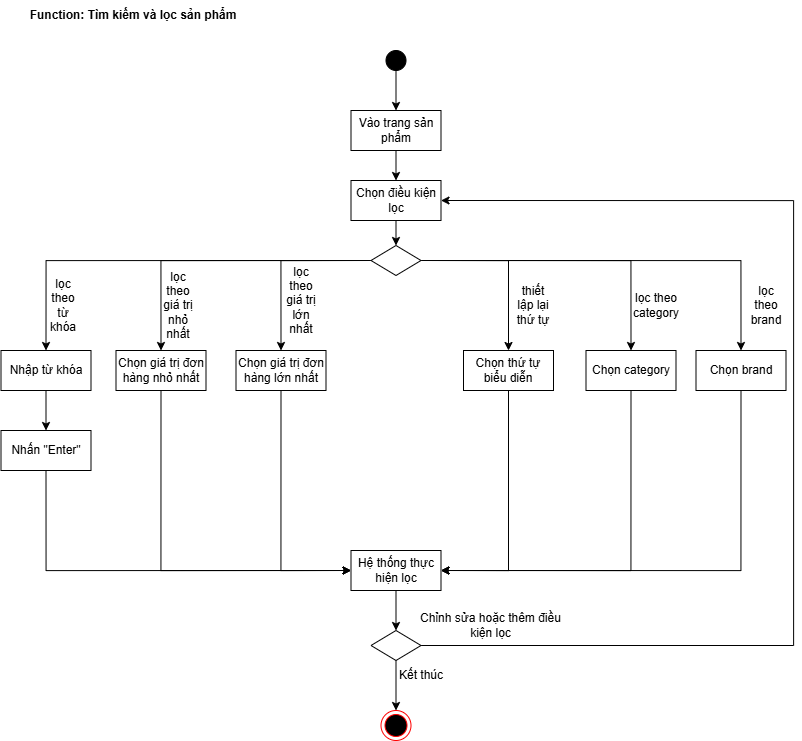
\includegraphics[width=0.8\textwidth]{images/chap8/fr/filter.png}
\vspace{0.7cm}
\caption{Sơ đồ luồng nghiệp vụ tính năng tìm kiếm và lọc sản phẩm}
\label{fig:flow_filter}
\end{figure}

Dựa trên các luồng xử lý tại Hình \ref{fig:flow_filter}, danh sách các ca kiểm thử chi tiết cho tính năng tìm kiếm và lọc sản phẩm được tổng hợp tại Bảng \ref{tab:tc_filter_full} nhằm xác minh tính chính xác của dữ liệu trả về.

\begin{table}[H]
\centering
\caption{Các ca kiểm thử chi tiết tính năng Tìm kiếm và lọc sản phẩm}
\label{tab:tc_filter_full}
\small
\begin{tabularx}{\textwidth}{|l|X|X|X|c|}
\hline
\textbf{ID} & \textbf{Tên kiểm thử} & \textbf{Mô tả kịch bản} & \textbf{Kết quả mong đợi} & \textbf{Trạng thái} \\ \hline
TC-005-001 & Tìm kiếm từ khóa & Nhập từ khóa vào ô tìm kiếm và nhấn Enter & Danh sách hiển thị sản phẩm có tên hoặc mô tả chứa từ khóa & Passed \\ \hline
TC-005-002 & Lọc giá tối thiểu & Chọn mức giá thấp nhất tại bộ lọc & Hệ thống chỉ hiển thị sản phẩm có đơn giá lớn hơn hoặc bằng mức chọn & Passed \\ \hline
TC-005-003 & Lọc giá tối đa & Chọn mức giá cao nhất tại bộ lọc & Hệ thống chỉ hiển thị sản phẩm có đơn giá nhỏ hơn hoặc bằng mức chọn & Passed \\ \hline
TC-005-004 & Sắp xếp danh sách & Lựa chọn các tiêu chí sắp xếp như giá hoặc ngày tạo & Danh sách sản phẩm được thay đổi thứ tự hiển thị đúng theo yêu cầu & Passed \\ \hline
TC-005-005 & Lọc theo danh mục & Chọn một loại sản phẩm cụ thể trên menu & Chỉ các sản phẩm thuộc danh mục đã chọn mới xuất hiện trên màn hình & Passed \\ \hline
TC-005-006 & Lọc theo nhãn hàng & Lựa chọn thương hiệu sản phẩm mong muốn & Kết quả trả về đúng với thương hiệu người dùng đã yêu cầu lọc & Passed \\ \hline
TC-005-007 & Kết hợp giá và hãng & Thiết lập khoảng giá kèm theo thương hiệu cụ thể & Sản phẩm hiển thị phải thỏa mãn đồng thời cả điều kiện giá và nhãn hàng & Passed \\ \hline
TC-005-008 & Kết hợp danh mục và từ khóa & Tìm kiếm từ khóa bên trong một danh mục nhất định & Kết quả trả về thuộc đúng danh mục và có chứa từ khóa tìm kiếm & Passed \\ \hline
TC-005-009 & Kết hợp nhiều tiêu chí & Lọc theo danh mục và giá kèm sắp xếp kết quả & Dữ liệu hiển thị đúng danh mục và khoảng giá theo thứ tự sắp xếp chọn lọc & Passed \\ \hline
TC-005-010 & Áp dụng tất cả bộ lọc & Thiết lập toàn bộ các tiêu chí lọc hiện có & Hệ thống xử lý chính xác và trả về kết quả thỏa mãn mọi ràng buộc & Passed \\ \hline
TC-005-011 & Từ khóa không tồn tại & Tìm kiếm với một chuỗi ký tự không có trong dữ liệu & Hệ thống thông báo không tìm thấy sản phẩm phù hợp với tiêu chí & Passed \\ \hline
TC-005-012 & Sai biệt hãng và danh mục & Kết hợp nhãn hàng và danh mục không có sản phẩm & Màn hình hiển thị thông báo không có kết quả phù hợp & Passed \\ \hline
TC-005-013 & Giá tối đa thấp hơn tối thiểu & Thiết lập mức giá tối đa nhỏ hơn mức tối thiểu & Hệ thống xử lý logic và không trả về sản phẩm nào hoặc báo lỗi lọc & Passed \\ \hline
TC-005-014 & Giá tối thiểu cao hơn tối đa & Điều chỉnh giá tối thiểu vượt quá giới hạn giá tối đa & Hệ thống đảm bảo tính nhất quán và yêu cầu điều chỉnh lại khoảng giá & Passed \\ \hline
\end{tabularx}
\end{table}

\subsubsection{Tính năng thêm sản phẩm vào giỏ hàng và đặt hàng}

Đây là luồng nghiệp vụ trọng tâm kết nối trực tiếp giữa các dịch vụ sản phẩm và kho hàng. Quy trình này bao gồm ba giai đoạn chính là thêm sản phẩm vào hệ thống lưu trữ tạm thời, điều chỉnh số lượng hàng hóa và thực hiện khởi tạo đơn hàng chính thức. Các sơ đồ dưới đây mô tả chi tiết các bước thực hiện và các nhánh rẽ logic tương ứng với từng giai đoạn.

\begin{figure}[H]
\centering
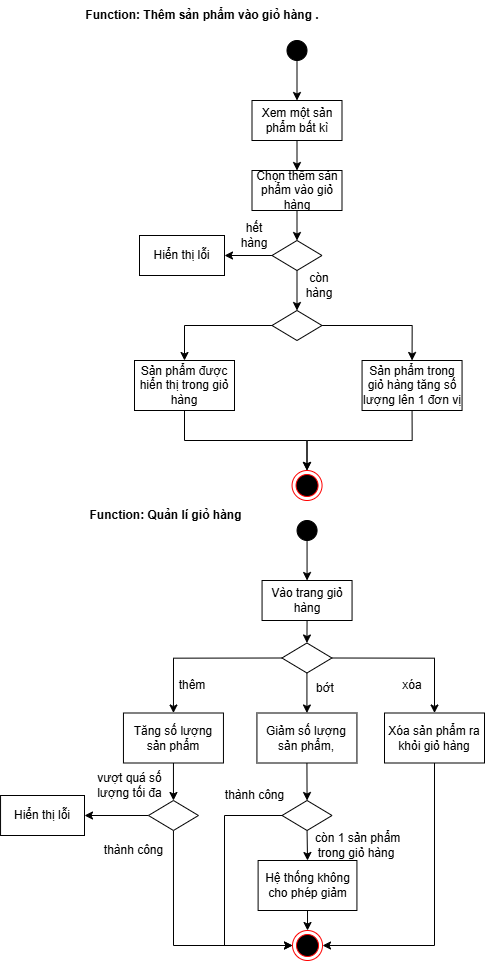
\includegraphics[width=0.7\textwidth]{images/chap8/fr/add-to-cart.png}
\vspace{0.7cm}
\caption{Sơ đồ luồng nghiệp vụ Thêm sản phẩm và Quản lý giỏ hàng}
\label{fig:flow_cart}
\end{figure}

\begin{figure}[H]
\centering
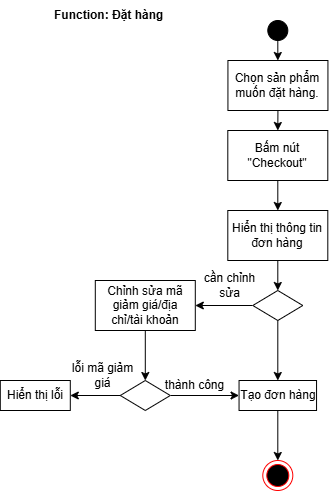
\includegraphics[width=0.5\textwidth]{images/chap8/fr/checkout.png}
\vspace{0.7cm}
\caption{Sơ đồ luồng nghiệp vụ Đặt hàng}
\label{fig:flow_checkout}
\end{figure}

Dựa trên các quy trình tại Hình \ref{fig:flow_cart} và Hình \ref{fig:flow_checkout}, danh sách các ca kiểm thử dưới đây được thiết lập để xác minh tính chính xác của dữ liệu khi luân chuyển qua các trạng thái khác nhau trong chu trình mua sắm.

Bảng \ref{tab:tc_cart_checkout_full} dưới đây là danh mục mô tả các kịch bản kiểm thử chi tiết cho quy trình này. Các ca kiểm thử được thiết kế để xác minh tính chính xác của dữ liệu khi người dùng thực hiện thay đổi số lượng hàng hóa và áp dụng các chính sách khuyến mãi trong giai đoạn thanh toán.

\begin{table}[H]
\centering
\caption{Các ca kiểm thử quy trình Quản lý giỏ hàng và Đặt hàng}
\label{tab:tc_cart_checkout_full}
\small
\begin{tabularx}{\textwidth}{|l|X|X|X|c|}
\hline
\textbf{ID} & \textbf{Tên kiểm thử} & \textbf{Mô tả kịch bản} & \textbf{Kết quả mong đợi} & \textbf{Trạng thái} \\ \hline
\multicolumn{5}{|l|}{\textbf{Giai đoạn 1: Thêm vào giỏ hàng}} \\ \hline
TC-007-001 & Sản phẩm hết hàng & Thêm sản phẩm có số lượng tồn kho bằng không. & Hệ thống hiển thị thông báo lỗi và từ chối thao tác. & Passed \\ \hline
TC-007-002 & Thêm sản phẩm mới & Thêm sản phẩm còn hàng chưa có trong giỏ. & Bản ghi mới được tạo với số lượng mặc định là một. & Passed \\ \hline
TC-007-003 & Sản phẩm hiện hữu & Thêm sản phẩm đã tồn tại sẵn trong giỏ hàng. & Hệ thống tự động tăng số lượng sản phẩm lên một đơn vị. & Passed \\ \hline
\multicolumn{5}{|l|}{\textbf{Giai đoạn 2: Quản lý giỏ hàng}} \\ \hline
TC-007-004 & Tăng số lượng thành công & Nhấn nút tăng số lượng khi còn đủ hàng tồn kho. & Số lượng cập nhật và tổng giá trị giỏ hàng tăng chính xác. & Passed \\ \hline
TC-007-005 & Tăng số lượng thất bại & Tăng số lượng vượt quá khả năng cung ứng của kho. & Hệ thống ngăn chặn hành động và hiển thị cảnh báo lỗi. & Passed \\ \hline
TC-007-006 & Giảm số lượng thành công & Nhấn nút giảm khi sản phẩm đang có từ hai món trở lên. & Số lượng giảm đi một đơn vị và tổng tiền cập nhật đúng. & Passed \\ \hline
TC-007-007 & Giảm số lượng thất bại & Giảm số lượng sản phẩm xuống dưới mức tối thiểu là một. & Hệ thống không thực thi lệnh giảm hoặc yêu cầu xóa món hàng. & Passed \\ \hline
TC-007-008 & Xóa sản phẩm & Sử dụng chức năng loại bỏ sản phẩm ra khỏi giỏ. & Sản phẩm bị xóa hoàn toàn khỏi danh sách chờ mua. & Passed \\ \hline
\multicolumn{5}{|l|}{\textbf{Giai đoạn 3: Thanh toán và Đặt hàng}} \\ \hline
TC-007-009 & Thanh toán tiêu chuẩn & Đặt hàng với thông tin mặc định không thay đổi. & Đơn hàng khởi tạo thành công và lưu trữ vào cơ sở dữ liệu. & Passed \\ \hline
TC-007-010 & Mã giảm giá hết hạn & Áp dụng mã Voucher đã quá thời hạn sử dụng. & Hệ thống từ chối áp dụng và yêu cầu kiểm tra lại mã. & Passed \\ \hline
TC-007-011 & Mã giảm giá hết lượt & Áp dụng mã Voucher đã đạt giới hạn số lần sử dụng. & Hệ thống báo lỗi mã không còn hiệu lực sử dụng. & Passed \\ \hline
TC-007-012 & Mã không tồn tại & Nhập chuỗi ký tự mã giảm giá sai lệch. & Hệ thống thông báo mã không hợp lệ hoặc không tìm thấy. & Passed \\ \hline
TC-007-013 & Thay đổi thông tin & Cập nhật địa chỉ hoặc ghi chú trước khi đặt hàng. & Đơn hàng ghi nhận chính xác các thông tin mới nhất. & Passed \\ \hline
\end{tabularx}
\end{table}

\subsubsection{Tính năng thanh toán đa phương thức}

Tính năng thanh toán đa phương thức cho phép người dùng linh hoạt lựa chọn giữa các hình thức giao dịch truyền thống và trực tuyến giả lập. Quy trình này xác minh khả năng xử lý của hệ thống khi tiếp nhận các phương thức thanh toán khác nhau và đảm bảo trạng thái đơn hàng được cập nhật chính xác sau khi giao dịch hoàn tất.

\begin{figure}[H]
\centering
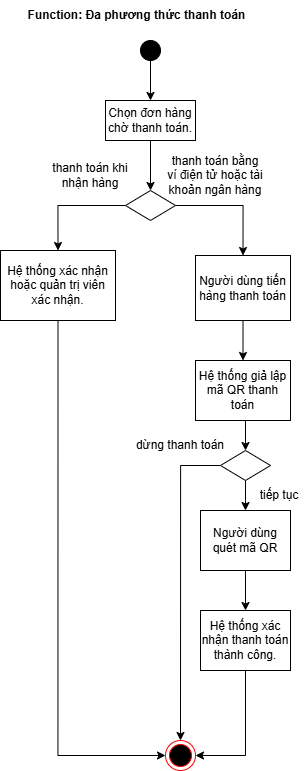
\includegraphics[width=0.4\textwidth]{images/chap8/fr/payment.png}
\vspace{0.7cm}
\caption{Sơ đồ luồng nghiệp vụ tính năng Thanh toán đa phương thức}
\label{fig:flow_payment}
\end{figure}

Dưới đây là mô tả các kịch bản kiểm thử nhằm đánh giá tính đúng đắn của luồng thanh toán giả lập cũng như khả năng xử lý các tình huống hủy bỏ giao dịch từ phía người dùng.

\begin{table}[H]
\centering
\caption{Các ca kiểm thử tính năng Thanh toán đa phương thức}
\label{tab:tc_payment}
\small
\begin{tabularx}{\textwidth}{|l|X|X|X|c|}
\hline
\textbf{ID} & \textbf{Tên kiểm thử} & \textbf{Mô tả kịch bản} & \textbf{Kết quả mong đợi} & \textbf{Trạng thái} \\ \hline
TC-008-001 & Phương thức COD & Lựa chọn hình thức thanh toán khi nhận hàng và xác nhận đơn. & Hệ thống ghi nhận phương thức COD và chuyển đơn hàng sang trạng thái chờ xác nhận. & Passed \\ \hline
TC-008-002 & Hủy thanh toán trực tuyến & Lựa chọn thanh toán mã QR nhưng thực hiện hủy bỏ giao dịch. & Hệ thống dừng quy trình thanh toán an toàn và giữ nguyên trạng thái chờ của đơn hàng. & Passed \\ \hline
TC-008-003 & Thanh toán trực tuyến thành công & Thực hiện quét mã QR giả lập và xác nhận hoàn tất giao dịch trực tuyến. & Hệ thống xác nhận thanh toán thành công và cập nhật trạng thái đơn hàng đã thanh toán. & Passed \\ \hline
\end{tabularx}
\end{table}

\subsubsection{Tài liệu quản lý kiểm thử chi tiết}

Toàn bộ các bước thực hiện cụ thể và các trường hợp kiểm thử mở rộng cho toàn bộ hệ thống được lưu trữ tại tệp tin dưới đây:

Truy cập tài liệu chi tiết tại: \href{https://docs.google.com/spreadsheets/d/1mHcj2cuIYbw-0h5_UOIEGGMhs_ll_Lcr/edit?usp=sharing&ouid=108057400976358149425&rtpof=true&sd=true}{Google Sheet}

